% !TeX spellcheck = pl_PL
% 
\newpage\section{Zarys idei systemu \textsl{\NazwaSys}}\label{sec:ideasystemu}
W rozdziale zostanie opisana pokrótce idea systemu \NazwaSys. Projekt składa się z 5 składowych: urządzenia sterującego (zarządzającego otwieraniem /zamykaniem drzwi), modułu zliczającego osoby, aplikacji mobilnej dedykowanej dla systemu Android oraz serwera operującego na bazie danych. Każdy z podsystemów zostanie przedstawiony, w jaki sposób ma funkcjonować, aby przybliżyć działanie systemu względem poszczególnych aktorów systemu (użytkowników, urządzeń).

\subsection{Schemat ideowy systemu \textsl{\NazwaSys}}
System łączy ze sobą 5 podsystemów różnymi interfejsami komunikacyjnymi.Urządzenia mobilne komunikują się z urządzeniem sterującym poprzez protokół bluetooth, a pozostałe połączenia oparte są na Ethernecie. Schemat połączeń urządzeń znajduje się na Rys. \ref{Schemat ogólny systemu}.

\begin{figure}[!h]
	\centering
	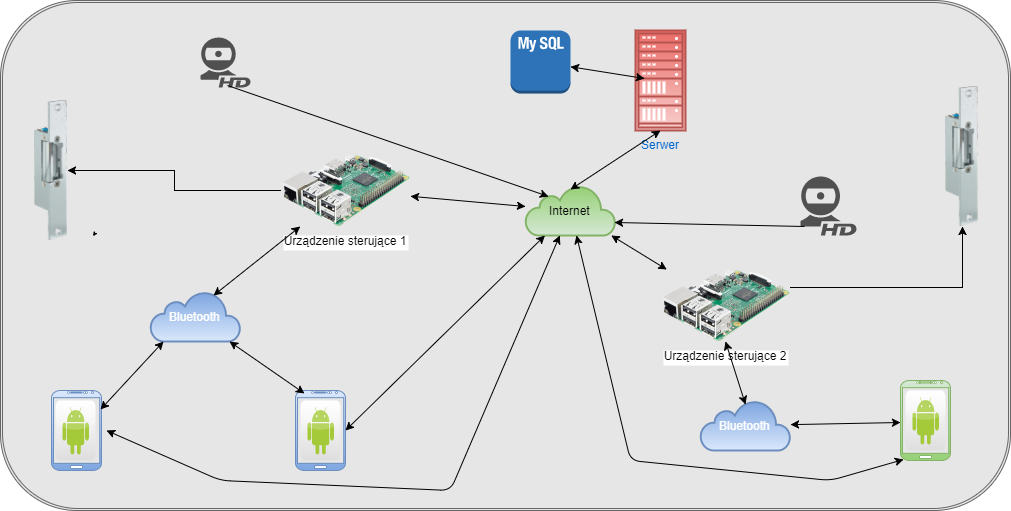
\includegraphics[width=15cm]{Obrazy/Schemat_ogolny}
	\caption{Schemat ogólny systemu}
	\label{Schemat ogólny systemu}
\end{figure}

Urządzenia sterujące łączą się z elektrozamkiem lub serwomechanizmem poprzez przewody elektryczne, natomiast z~kamerą IP oraz serwerem poprzez sieć LAN. Aplikacja serwerowa nawiązuje połączenie z bazą danych przez lokalny interfejs sieciowy.

\subsection{Opis składowych systemu}
System ma złożoną budowę, ponieważ składa się z 5 podsystemów. Pierwszym z nich jest urządzenie sterujące, w którego skład wchodzą Raspberry Pi~3\footnote{ Raspberry Pi 3 jest mikrokomputerem z procesorem ARMv7} oraz serwomechanizm lub zamek elektroniczny. Podstawową funkcją tego modułu jest weryfikacja klucza cyfrowego, przesyłanego przez urządzenia mobilne oraz otwieranie zamka przy pozytywnym wyniku weryfikacji. Każde zdarzenie zapisywane jest w pliku z logami. Oprogramowanie mikrokomputera obejmuje system Linux raspbian-jessie \footnote{ System operacyjny raspbian-jessie jest dedykowanym systemem operacyjnym dla komputerów Raspberry Pi umożliwiającym w pełni wykorzystać interfejsy wejścia wyjścia} oraz skrypt napisany w języku Python 2.7. Programy łączą się do serwera w celu pobrania informacji o poprawności i~dacie ważności certyfikatu dostępowego, następnie dane są porównywane z~tymi otrzymanymi od użytkownika. Dodatkowo weryfikowany jest podpis cyfrowy, którym sygnowany jest klucz dostępowy. Jeśli dane zostaną zweryfikowane poprawnie, to zostaje wysterowany serwomechanizm (lub wysłany impuls do elektrozamka), który otwiera zamek. W przeciwnym przypadku użytkownik zostanie poinformowany o odmowie dostępu, a nieudana próba dostania się do~systemu zarejestrowana zostanie w bazie danych wraz z danymi właściciela klucza dostępowego.

Drugim elementem jest aplikacja mobilna napisana na platformę Android w wersji minimalnej 5.0. Program ma na celu przechowywanie w pamięci smartphona kluczy cyfrowych (dostępowych) użytkownika oraz umożliwienie interakcji użytkownika z systemem.

Kolejnym z elementów jest aplikacja serwerowa wraz ze stroną internetową. Rolą serwera w tym systemie jest pośredniczenie w operacjach na danych dostępowych w bazie danych MySQL. Dodatkowo serwer obsługuje stronę internetową, która wyświetla na bieżąco historię użycia zamków w systemie.

Przedostatnim elementem składowym systemu jest baza danych, która przechowuje wszystkie kluczowe informacje systemu oraz udostępnia je serwerowi.

Ostatnim ze składowych systemu jest oprogramowanie zliczające liczbę osób wchodzących i wychodzących dla danego pomieszczeniu lub całego budynku wraz z kamerą, której zadaniem jest obliczanie informacji o~aktualnej liczbie osób w danym pomieszczeniu. 

\subsection{Podmioty systemu} 
W pracy dyplomowej można wyodrębnić następujące podmioty:
	\begin{itemize}
	\item {Użytkownik niezalogowany} --- jest to użytkownik, który posiada aplikacje mobilną na swoim urządzeniu, lecz nie wykonał procesu logowania,
	\item {Użytkownik niezarejestrowany} --- jest to użytkownik który wysłał prośbę o zarejestrowanie, lecz nie została ona jeszcze zatwierdzona przez administratora,
	\item {Użytkownik zalogowany} --- jest to użytkownik, który przeszedł poprawnie proces logowania, posiada on ograniczoną funkcjonalność aplikacji,
	\item {Administrator} --- jest to użytkownik zalogowany, który posiada uprawnienia administratora, co wiąże się z pełnym dostępem do funkcji aplikacji mobilnej (zawiera funkcje użytkownika zalogowanego),
	\item {Aplikacja serwerowa} --- jest to oprogramowanie, zarządzające całym systemem oraz pośredniczące w przekazywaniu informacji z bazy danych,
	\item {Urządzenie sterujące} --- jest to oprogramowanie zarządzające dostępem fizycznym do pomieszczeń,
	\item {Elektrozamek} --- urządzenie umieszczone w futrynie drzwi, pozwalające sterować stanem otwarcia zamka,
	\item {Serwomechanizm} --- silnik krokowy, nakładka na zamek fizyczny w drzwiach, sterujący ryglem w futrynie,
	\item {Moduł zliczania osób} --- jest to oprogramowanie zwracające w czasie rzeczywistym ilość osób przebywających w danym pomieszczeniu,
	\item {Kamera IP} --- urządzenie wizyjne, udostępniające obraz do celów zliczania osób.
\end{itemize}